
\chapter{Appendix}
\label{chap:Appendix}
The appendix offers data used throughout the document in further detail.



\section{Data regarding gaming devices}

\textbf{First}, the data relevant for used devices from \cite[7]{LimelightNetworks.2020} is shown in relative measures (Figure \ref{fig:GameingDeviceDataTable}).
\begin{figure}
	\centering{
		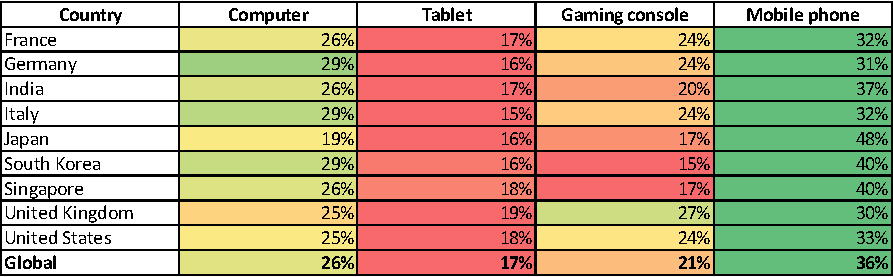
\includegraphics[width=.90\linewidth,keepaspectratio=true]{contents/images/GameingDeviceData}
		\caption{Share of devices by gaming time \cite[7]{LimelightNetworks.2020}}
		\label{fig:GameingDeviceDataTable}
	}
\end{figure}

\noindent \textbf{Second}, a chart from 'Counterpoint Research' by \cite{Wang.2021} is given (Figure \ref{fig:GameingDeviceStorageSpace}),
which supports the claim that "Average Smartphone NAND Flash Capacity Crossed 100GB in 2020".

\begin{figure}
	\centering{
		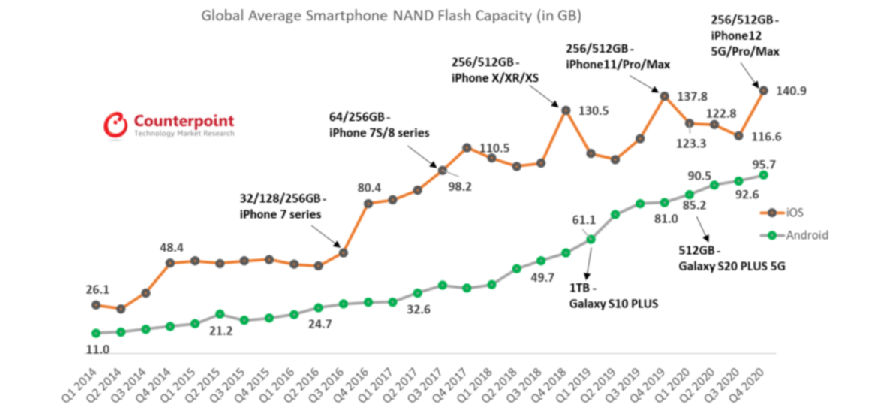
\includegraphics[width=.90\linewidth,keepaspectratio=true]{contents/images/GameingDeviceStorageSpace}
		\caption{Average smartphone storage space (From \cite{Wang.2021})}
		\label{fig:GameingDeviceStorageSpace}
	}
\end{figure}

\noindent \textbf{Third}, the data relevant for game characteristics from \cite[18]{LimelightNetworks.2020} is shown in relative measures (Figure \ref{fig:GameCharacteristicsDataTable}).

\begin{figure}
	\centering{
		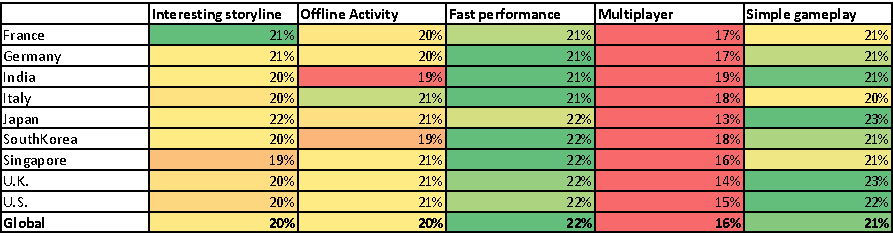
\includegraphics[width=.90\linewidth,keepaspectratio=true]{contents/images/GameCharacteristicsData}
		\caption{Game characteristics data \cite[18]{LimelightNetworks.2020}}
		\label{fig:GameCharacteristicsDataTable}
	}
\end{figure}



\section{Scripts for graph's plots}
\label{script:GraphPlots}

\subsection{Plot: BFT shuffling cards}
\label{script:BFTshufflingCards}
Python code for figure \ref{fig:ShuffleCards}, '\textit{BFT shuffling cards}':
\pythonexternal{contents/graphsplots/ShufflePlot.py}
\pagebreak

\subsection{Plot: General storage allocation}
\label{script:GeneralStorageAllocation}
Python code for figure \ref{fig:StorageAllocation_Base}, '\textit{General \gls{BT} storage allocation chart}':
\pythonexternal{contents/graphsplots/BCstorageAllocationBase.py}
\pagebreak

\subsection{Plot: Storage allocation Prune procedure/Child-chain}
\label{script:StorageAllocationPPSC}
Python code for figure \ref{fig:StorageAllocationPrune}, '\textit{Prune procedure/Child-chain chart}':
\pythonexternal{contents/graphsplots/storageAllocationPruneSC.py}
\pagebreak

\subsection{Plot: Storage allocation Meta State Block}
\label{script:StorageAllocationMetaState}
Python code for figure \ref{fig:StorageAllocation_MetaState}, '\textit{Meta-State Block chart}':
\pythonexternal{contents/graphsplots/storageAllocationMetaState.py}
\pagebreak

\subsection{Plot: Storage allocation comparison}
\label{script:StorageAllocationComp}
Python code for figure \ref{fig:BC_StorageAllocation_All_Big}, '\textit{Storage allocation comparison}':
\pythonexternal{contents/graphsplots/BCstorageAllocationAllBig.py}

